
\chapter{La mise en \oe{}uvre de l'API}
\label{implementation.chap}

\subsection{Pipeline}

Mentionn\'e au chapitre ant\'erieur, le pipeline est compos\'e d'une cha\^ine de traitement appel\'e \TT{Pipe}. Un \TT{Pipe} est repr\'esent\'ee essentiellement par une s\'erie d'op\'erateurs d\'efinis par l'utilisateur qui sont appliqu\'es aux \'el\'ements d'un flux. \TT{PpFf} est impl\'ement\'e au-dessus de la biblioth\`eque \TT{FastFlow}, de sorte que nous utilisons \TT{ff\_node}, \TT{ff\_pipeline} et \TT{ff\_farm} comme fournisseur pour l'ex\'ecution de \TT{PpFf}. 

D\'ecrits dans le chapitre pr\'ec\`edent, les op\'erateurs qui composent un \TT{Pipe} sont de deux types : les op\'erateurs sans \'etat et les op\'erateurs avec l'\'etat. Comme nous pouvons le voir dans la figure~\ref{MapToFastFlow.fig} un op\'erateur h\'erite de la class \TT{ff\_node} de \TT{FastFlow}. Le \TT{Pipe} contient un ou plusieurs op\'erateurs sans \'etat et un seul op\'erateur avec \'etat. Lorsque ce dernier est ajout\'e dans le \TT{pipeline}, la m\'ethode \TT{run()} est appel\'ee. \`A ce stade, un objet de type \TT{ff\_pipeline} correspondant au \TT{Pipe} est cr\'e\'e. Ensuite, chaque op\'erateur d\'efini par l'utilisateur est visit\'e et en fonction de la configuration \'etablie, des objets de type \TT{ff\_node} ou \TT{ff\_farm} sont ajout\'es comme stage au \TT{ff\_pipeline}. Chaque nœud ainsi ajout\'e dans \TT{ff\_pipeline}, sera ex\'ecut\'e dans un fil d'ex\'ecution.
La cr\'eation de \TT{Pipe} est r\'ealis\'ee \`a l'aide de \TT{PipeManager}.

\begin{figure}[ht]
\centering
     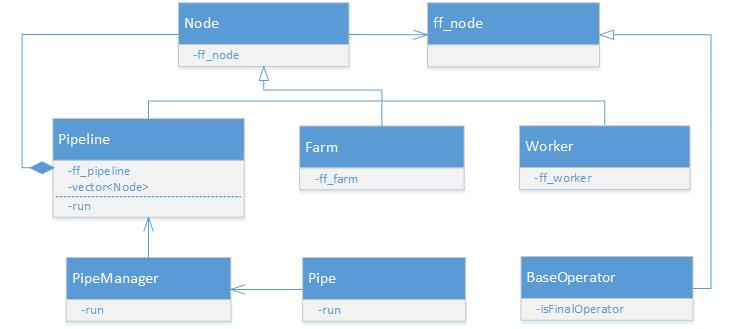
\includegraphics[width=1.0\textwidth]{Figures/MapToFastFlow.jpg}
      \caption{Le mappage de \TT{PpFf} \`a \TT{FastFlow}.}
       \label{MapToFastFlow.fig}
\end{figure}


\subsection{Parall\'elisation}

La cr\'eation du code parall\`ele a \'et\'e le domaine des experts. La complexit\'e du code parall\`ele diminue la productivit\'e, ce qui peut augmenter les co\^uts de d\'eveloppement. \TT{PpFf} permet aux programmeurs de composer du code s\'equentiel et de l'ex\'ecuter en parall\`ele. Dans une interface unique, l'\TT{API} offre deux mod\`eles de parall\'elisme : le parall\'elisme de flux et \TT{Task-Farm}.


\subsubsection{Parall\'elisme de flux}

Le parall\'elisme de flux consiste \`a ex\'ecuter plusieurs \'etapes d'un traitement s\'equentiel en parall\`ele en leur faisant traiter des données diff\`erentes. Les donn\'ees se succ\`edent ainsi les unes aux autres dans les diff\'erentes \'etapes, nomm\'ees aussi des stages. Le traitement effectu\'e dans un stage \`a un instant donn\'e peut d\'ependre des traitements effectu\'es par ce stage pour les donn\'ees pr\'ec\'edentes. Ce fonctionnement permet de parall\'eliser des traitements avec de fortes d\'ependances entre les donn\'ees sans avoir recours \`a de nombreuses synchronisations. 
Un flux avec n stages peut \^etre formellement exprim\'e sous la forme d'une composition s\'equentielle d'op\'erateurs sur les \'el\'ements d'entr\'ee. 

\[
	O(x) = O_n( \ldots (O_k( \ldots O_1(x)) \ldots ) \ldots ));
\]

Dans ce cas, la parall\'elisation est repr\'esent\'ee par un graphique lin\'eaire de n travailleurs. Chaque travailleur correspond \`a une op\'eration sp\'ecifique. La figure~\ref{ParallelismeDuFlux.fig} montre la repr\'esentation graphique du parall\'elisme de flux. Cette solution n'acc\'el\`ere pas le calcul d'un seul \'el\'ement. Par contre, elle am\'eliore le d\'ebit de sortie.

\begin{figure}[ht]
\centering
     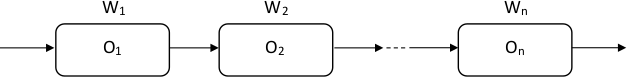
\includegraphics[width=1.0\textwidth]{Figures/ParallelismeDuFlux.jpg}
      \caption{Le parall\'elisme de flux.}
       \label{ParallelismeDuFlux.fig}
\end{figure}


\subsubsection{Task-Farm}

Le mod\`ele \TT{Task-Farm} impl\'ement\'e dans \TT{PpFf}  consiste \`a r\'epliquer un op\'erateur parmi un ensemble de travailleurs identiques. Autrement dit, il vise \'a effectuer un traitement identique sur un ensemble de donn\'ees ind\'ependantes les unes des autres. \TT{Task-Farm} est compos\'e de trois principales entit\'es : \TT{Emitter}, \TT{Collector} et multiple travailleurs. L'\TT{Emitter} distribue les \'el\'ements d'entr\'ee aux travailleurs selon une certaine politique d'ordonnancement afin d'\'equilibrer la charge des travailleurs. La figure~\ref{ParallelismeTaskFarm.fig} montre le mod\`ele \TT{TaskFat} impl\'ement\'e dans \TT{PpFf}. Les \'el\'ements sont repartis aux travailleurs selon le mod\`ele \TT{round robin}. Les travailleurs re\c coivent les \'el\'ements d'entr\'ee et appliquent sur chacun d'eux l'op\'erateur d\'efini au pr\'ealable par l'utilisateur. Les r\'esultats sont envoy\'es vers le collecteur charg\'e de les collecter et de les transmettre au flux de sortie.

L'impl\'ementation parall\`ele de ce mod\`ele peut \^etre formellement exprim\'ee sous la forme d'un ensemble de travailleurs 

\[
	{W_1, W_2,\ldots, W_n}
\]

qui applique l'op\'erateur 

\[
	O : X -> Y
\]

sur les \'el\'ements Xn apparaissant dans le flux d'entr\'ee. Le r\'esultat Yi est g\'en\'er\'e en appliquant l'op\'erateur O sur l'\'el\'ement Xi. L'op\'eration sera ex\'ecut\'ee en parall\`ele par les diff\'erents travailleurs. Dans ce cas, la structure du mod\`ele d'ex\'ecution peut \'eventuellement recevoir, en param\`etre, le nombre de travailleurs \`a utiliser pour l'ex\'ecution parall\`ele. Si ce param\`etre n'est pas renseign\'e, l'interface prend un seul travailleur d\'efini par d\'efaut. Cette solution est capable d'augmenter le d\'eit du traitement des donn\'ees, c'est \`a dire le nombre de donn\'ees qui peuvent \^etre trait\'ees en un temps donn\'e.

\begin{figure}[ht]
\centering
     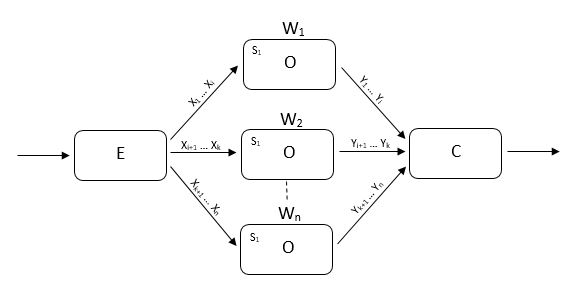
\includegraphics[width=1.0\textwidth]{Figures/ParallelismeTaskFarm.jpg}
      \caption{Task Farm}
       \label{ParallelismeTaskFarm.fig}
\end{figure}








\subsection{Stages}

Le traitement du flux de donn\'ees est mod\'elis\'e en utilisant une cha\^{\i}ne d'\'etapes. Dans notre API, une \'etape est repr\'esent\'ee par un \texttt{Stage}, et chaque \texttt{Stage} est compos\'e d'un ou plusieurs op\'erateurs. Notons toutefois que ce module n'est pas visible \`a l'utilisateur. 


\GT{Donc, en lien avec ma remarque pr\'esent\'ee plus haut: si la
notion de Stage n'est pas visible \`a l'utilisateur, elle ne devrait
donc pas faire partie de la pr\'esentation de l'API. Elle devrait
plut\^ot \^etre trait\'ee dans la partie Mise en \oe{}uvre
(impl\'ementation).}
